\documentclass[conference]{IEEEtran}
\usepackage{multirow}
\usepackage{color}
\usepackage{adjustbox}
\usepackage{graphics}
\usepackage{graphicx}
\usepackage{rotating}
\usepackage{graphics}
\usepackage{colortbl}
\usepackage{picture}
\usepackage{algorithm}
\usepackage{algorithmicx}
\usepackage{algpseudocode}
\renewcommand{\algorithmicensure}{\textbf{Output:}}


\begin{document}
\title{CSC791 Spatial-Temporal Data Mining Project Report}
\author{Wei Fu, George Mathew, Qiang Zhang} 

\maketitle
\begin{abstract}
  Crater detection has been one fundamental task in planetary science, which has drawn great attention from fields of data mining and image processing. In this project, three typical spatial data mining algorithms for crater detection are discussed, implemented and analyzed. Based on this result, we propose to use SVM, Neural
networks, tuned-CART as well as ensemble method to do crater detection. Experimental results on the dataset which includes 7365 crater candidates demonstrate that probability of detection of tuned-CART can be up to 86.7\% and F score of ensemble method can be 83\%. The results also demonstrate that no single method can be good in all metric measures.
\end{abstract}

{\bf Keywords:} Crater Detection, Transfer Learning, Boost, CART, SVM, Neural Networks.

\section{Introduction}
Craters are key structures formed by the collisions of asteroid or comet with planetary surface. To investigate past and future geological information, craters detection methods or tools with high precision are demanded. Manual inspection of images is one mainly used method. However, due to the increasing huge amount of craters needed to be identified in very high resolution planetary images, this widely used method seems out-dated but automatic detection is the only practical solution to such tasks. Several reasons \cite{kim2005automated} can explain this:
\begin{itemize}
 \item The lighting conditions result in different qualities of the images, which would affect the detecting accuracy.
 \item Some geographical features, like volcanoes, have similar morphological characteristics as craters.
 \item Crater rims are frequently eroded due their formation millions of years ago. 
\end{itemize}

During past years, several methods have been invented and proposed to detect craters from data mining and image processing fields. In this project, our contributions can be summarized as follows:
    \begin{itemize}
    \item implement tree detection algorithms in \cite{ding2011subkilometer}.
    \item apply SVM, neural networks, and tuned-CART on the dataset to detect craters
    \item design a model to ensemble results from above methods and identify craters based on majority voting.
    \end{itemize}
% we're trying to learn and implement algorithms that address all these issues. We choose as a main reference to build a robust and practical crater detection framework. Based on this, a new detection algorithm will be designed to further improve the performance .

\section{Problem definition}
The automatic detection algorithms should solve the above challenges. Specifically, two problems are to address: (1) based on the candidates of craters, how to classify them accurately into crater and non-crater classes? (2) given a training dataset including crater and non-crater examples, how to make the algorithm applicable to detect the craters in other data sets.

\section{Related Work}

Salamuniccar\cite{salamuniccar2008open} provided an extensive review of previous work on crater detection algorithms, which can be divided into two categories: supervised and unsupervised-learning methods. 

The unsupervised approcahes identify crater rims in an image as circular or elliptical features\cite{bandeira2007impact,cheng2003optical,honda2002mining,leroy2001crater,galloway2014image}. All of the methods fall in this category would use Hough Transform or similar image processing methods to improve the performance of crater edge detection Specifically, in \cite{leroy2001crater}, a new robust method is proposed to infer curvature estimation from noisy space data  to compute a dense saliency map corresponding to the position and shape of the craters. The detected craters in the image are matched with the craters projected from a 3D model. Authors of \cite{bandeira2007impact} presented a methodology that brought number of techniques in the fields of image processing and pattern recognition, including candidate selection, template matching and final identification based on the probability to detect impact craters on images. Rie et al.\cite{honda2002mining} proposed to group original images according to spatial frequency patterns and both optimized parameters setts and noise reduction techniques used to identify candidate craters and false candidates are excluded using a self-organizing map approach.

Supervised methods are designed based on data mining techniques, where algorithms use the labeled data sets to train a learner and then identify craters on new data sets with this learner. Jinhao et al. \cite{Jihao2015selected} proposed to generate Gist feature from selected training samples and the crater detection is conducted using Gist feature vectors with random forests classification. Siyi et al.\cite{siyi2011image} used semi-supervised Active Class Selection algorithm to iteratively enrich an original small training set, without additional human labeling effort, to detect craters form a large volume of images. Ying et al. \cite{ying2013crater} proposed to integrate the Least Absolute Shrinkage and Selection Operator method  with Bayesian network classifier for this task. The work we mainly referred designed a framework, which used a supervised boosting learning algorithms and transfer learning methods to classify crater candidates based on the texture features extracted from the original images.


\section{Baseline Methods}
In this projects, we implemented tree algorithms, including Boost algorithm, Naive algorithm and Transfer Learning algorithm, proposed in \cite{ding2011subkilometer}.
\begin{figure}[!h]
\begin{center}
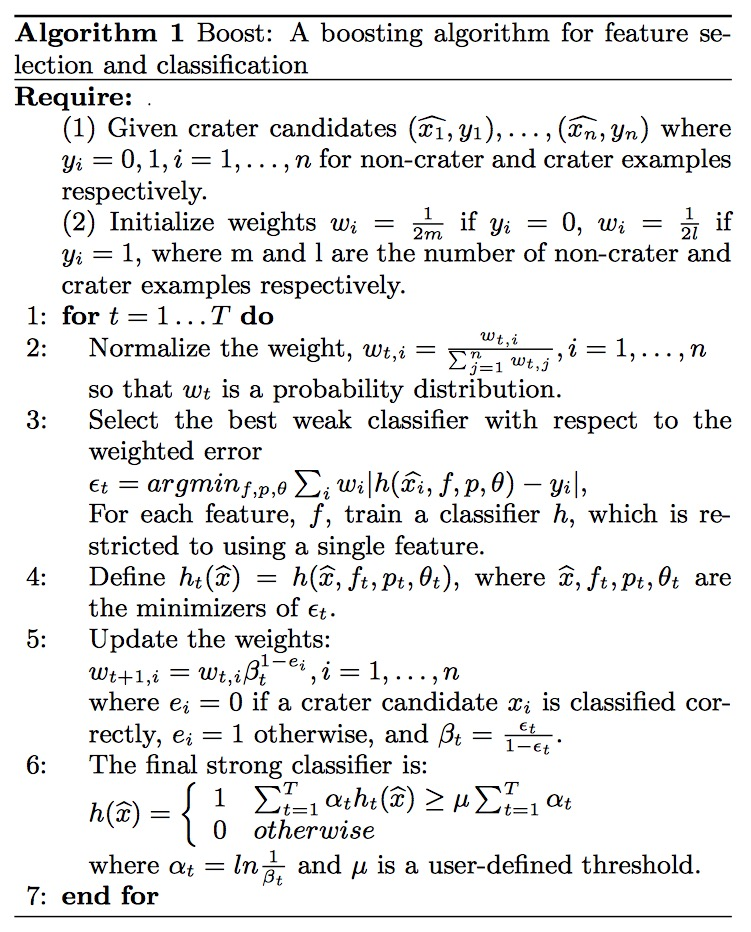
\includegraphics[scale=0.34]{boost.png}
\label{default}
\end{center}
\end{figure}

\begin{figure}[!htb]
\begin{center}
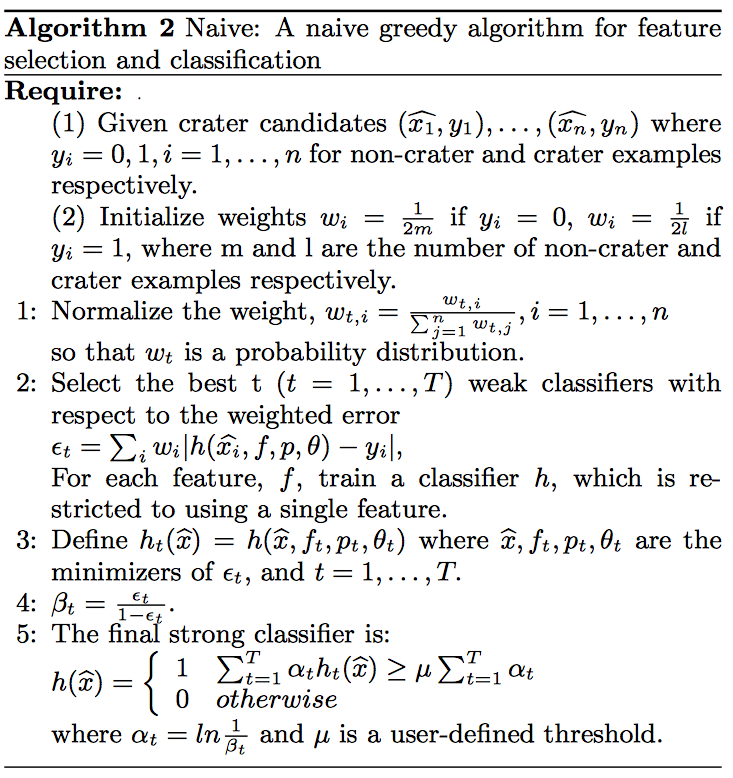
\includegraphics[scale=0.34]{naive.png}
\label{default}
\end{center}
\end{figure}

\begin{figure}[!hb]
\begin{center}
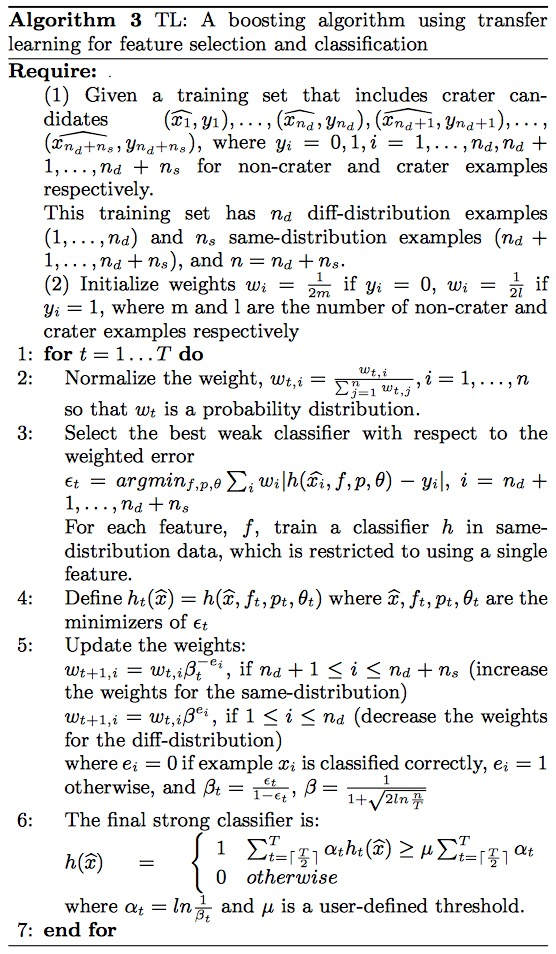
\includegraphics[scale=0.45]{TL.png}
\label{default}
\end{center}
\end{figure}

The Boost algorithm generates a sequence of weak classifers $h_t(f)$ and combine them through a weighted approach to build a strong classifier $H(\hat{x})$:
\begin{equation}
 H(\hat{x}) = \sum_{t=1}^{T}\alpha_th_t{f}
\end{equation},
where T is the number of iterations, $t = 1,...,T$, $\hat{x} = <f_1,...,f_N>$ is the feature vector that describes a crater candidate; $f \in {f_1,...,f_N}$ is the single feature used to construct a weak classifier $h_t(f)$ and $\alpha_t$ is the weight of hypothesis $h_t(f)$. The Boost algorithm iteratively selects one feature at a time and stops when reaching T iterations; each iteration the Boost algorithm will choose a best feature, which includes weak classifier learning , features selection and weight updating. More details are described in algorithm 1\cite{ding2011subkilometer}.


The Naive algorithm \cite{ding2011subkilometer} is to reduce the time complexity required by Boost algorithm. This algorithm uses the same weak classifier learning step and selects the top T best features using the weighted error sum in the step of feature selection as a criterion without any further iterations on weight updating.

The Transfer Learning algorithm has the same three steps as Boosting algorithm, but the weight updating step is different. In Boosting algorithm, both training and testing data sets are drawn independently and identically from an underlying distribution and it is not expected to perform well if the testing data has a different distribution from the training data. The method used here is to build the  strong classifier sequentially. Details are presented in {\it weight updating}step in Algorithm 3\cite{ding2011subkilometer}.


% \begin{figure*}[ht]
% \begin{center}
% 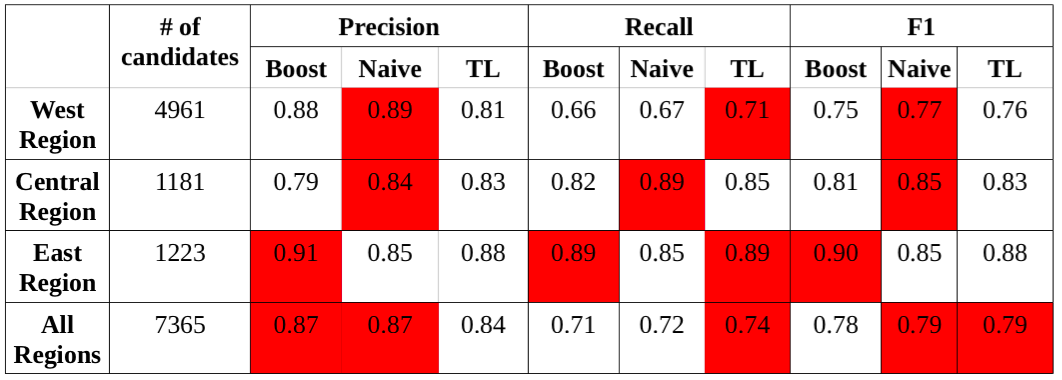
\includegraphics[scale=0.45]{T_50.png}
% \caption{Performance of Boost, Naive, and TL algorithms; T= 50; Boost: mu = 0.475; Naive: mu = 0.325; TL: mu = 0.5.}
% \label{T50}
% \end{center}
% \end{figure*}



% \begin{figure*}[ht]
% 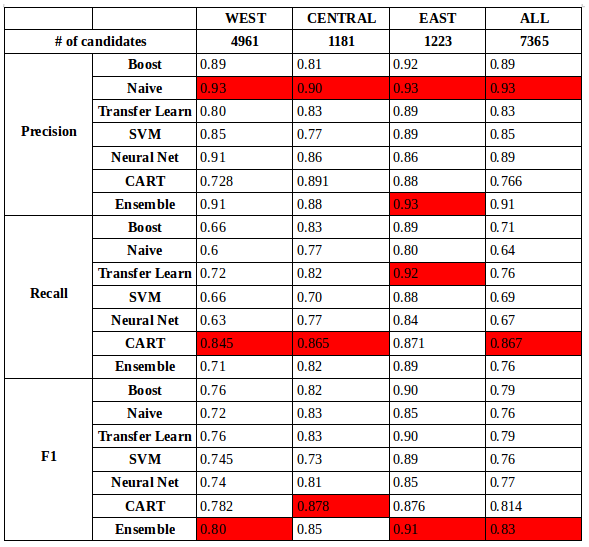
\includegraphics[scale=0.75]{all.png}
% \caption{Performance of All the algorithms; T= 150; Boost: mu = 0.475; Naive: mu = 0.325; TL: mu = 0.5.; SVM: kernel = polynomial, degree = 3; Neural Net: hidden layers = 250, learn rate = 0.01 }
% \label{ALL}
% \end{figure*}

\section{Proposed Methods}

\subsection{Support Vector Machines}
The crater data set can modeled into various kernels and then could be classified into craters or non-craters. Kernels project the attributes of the data set into higher dimensions that explain the features better. Few types of kernels we can choose from are "linear", "polynomial", "radial basis functions" and "sigmoid" kernels. Based on experiments of M.Ding et.al \cite{Ding2013385} order of the kernel does not make a significant improvement in the accuracy of the algorithm. Hence we chose a polynomial kernel of degree 3.

\subsection{Neural Networks}
Artificial Neural Networks(ANN) is a class of adaptive machine learning technique modeled after the human brain. It was one of the first algorithm employed for crater detection \cite{ding2011subkilometer} primarily due to its low false alarm rate. Neural networks can be modelled to contain multiple hidden layers and a varying learning rate. For our implementation of neural networks we used 250 hidden layers and a learning rate of 0.01. 

\subsection{Tuned CART}
One of the “black arts” of data mining is setting the tuning
parameters that control the choices within a data miner. The 
parameters used in data miners, like SVM, 
KNN and CART, have been well-explored by
the developers of those algorithms, in which case tuning
would not lead to large performance improvements. However, 
depending on different applications or distributions of the 
data sets, we do need to tune parameters using local data
sets to achieve better performance\cite{Wei2015ase}. 
Since the crater data sets used in this study have over thousand features,
we would expect a local data miner tuned by the local training data sets
are more helpful.

We consider to tune CART implemented in python\cite{scikit-learn} for 
this case study. In this python version of CART, we have {\it max\_feature, max\_depth,
min\_sample\_leaf} and {\it min\_sample\_split} parameters to be tuned.
As suggested by \cite{Wei2015ase}, Differential Evolution(DE), a light weight optimizer,
has been applied to tune these parameters. The pseudo code has been list in Algorithm \ref{alg:DE}.
For the space limitation, more details about tuning CART can be found in \cite{Wei2015ase}.
  
\setcounter{algorithm}{3}
\begin{algorithm}[!t]

\scriptsize

\begin{algorithmic}[1]
\Require $testData$,$trainData$,$tuneData$
\Ensure $results$


\Function{Tuned-CART}{$testData$,$trainData$,$tuneData$}
 \State $tunedParameters  \gets $ DE($tuneData$) 
 \State $model \gets $ fitCART($tunedParameters$,$trainData$)
 \State $results \gets $predict($model$,$testData$)
  \State \Return $results$
\EndFunction
        \end{algorithmic} 
\caption{Pseudocode for tuned-CART}
\label{alg:DE}
\end{algorithm}

\subsection{Ensemble}
Most methods employed have pros and cons of its own. For example the naive greedy method has high precision an really low recall. But CART has low precision and high recall. Hence, we build all the models and select the predicted value using a voting technique \cite{voting}. In the case of voting based methods, there is chance that there will be a tie. In such cases we randomly select between the classes. But in most cases there should not be ties.


\section{Experimental results}
\subsection{Dataset description}

The dataset used in this project is from the same source as \cite{ding2011subkilometer}, which is a portion of the High Resolution Stereo Camera nadir panchromatic image h0905. The selected image has the resolution of 12.5 meters/pixel and the size of 3,000 by 4,500 pixels. The image is divided into west region, central region and east region, which include $4961$,$1181$ and $1223$ crater candidates, respectively. For some unknown reason, these number are different from those in \cite{ding2011subkilometer} even though we got this data set from their website. Our implementation for the algorithm is available in our github repository(\url{http://goo.gl/SSQ5iq}).


\begin{figure*}[ht]
\renewcommand{\baselinestretch}{0.9}
\resizebox{\textwidth}{!}{
\centering
\scriptsize
\begin{tabular}{c|c|l|l|l|l|l|l|l|l|l|}
\cline{2-11}
\multicolumn{1}{l|}{\multirow{2}{*}{}}                                         & \multirow{2}{*}{\#of candidates} & \multicolumn{3}{c|}{Precision}       & \multicolumn{3}{c|}{Recall}                   & \multicolumn{3}{c|}{F1}                       \\ \cline{3-11} 
\multicolumn{1}{l|}{}                                                          &                                  & Boost         & Naive         & TL   & Boost         & Naive         & TL            & Boost         & Naive         & TL            \\ \hline
\multicolumn{1}{|c|}{\begin{tabular}[c]{@{}c@{}}West \\ Region\end{tabular}}   & 4961                             & 0.88          & \textbf{0.89} & 0.81 & 0.66          & 0.67          & \textbf{0.71} & 0.75          & \textbf{0.77} & 0.76          \\ \hline
\multicolumn{1}{|c|}{\begin{tabular}[c]{@{}c@{}}Central\\ Region\end{tabular}} & 1181                             & 0.79          & \textbf{0.84} & 0.83 & 0.82          & \textbf{0.89} & 0.85          & 0.81          & \textbf{0.85} & 0.83          \\ \hline
\multicolumn{1}{|c|}{\begin{tabular}[c]{@{}c@{}}East\\ Region\end{tabular}}    & 1223                             & \textbf{0.91} & 0.85          & 0.88 & \textbf{0.89} & 0.85          & \textbf{0.89} & \textbf{0.90} & 0.85          & 0.88          \\ \hline
\multicolumn{1}{|c|}{\begin{tabular}[c]{@{}c@{}}All\\ Regions\end{tabular}}    & 7365                             & \textbf{0.87} & \textbf{0.87} & 0.84 & 0.71          & 0.72          & \textbf{0.74} & 0.78          & \textbf{0.79} & \textbf{0.79} \\ \hline
\end{tabular}
}
\caption{Performance of Boost, Naive, and TL algorithms; T= 50; Boost: mu = 0.475; Naive: mu = 0.325; TL: mu = 0.5.}
\label{T50}

\end{figure*}
% Please add the following required packages to your document preamble:
% \usepackage{multirow}
\begin{figure*}[t]
\centering
\begin{adjustbox}{max width=\textwidth}
\begin{tabular}{|l|c|c|c|c|c|}
\hline
\multicolumn{2}{|c|}{\multirow{2}{*}{\# of candidate}}            & WEST          & CENTRAL       & EAST          & ALL           \\
\multicolumn{2}{|c|}{}                                            & 4961          & 1181          & 1223          & 7365          \\ \hline
\multicolumn{1}{|c|}{\multirow{7}{*}{Precision}} & Boost          & 0.89          & 0.81          & 0.92          & 0.89          \\ \cline{2-6} 
\multicolumn{1}{|c|}{}                           & Naive          & \textbf{0.93} & \textbf{0.90} & \textbf{0.93} & \textbf{0.93} \\ \cline{2-6} 
\multicolumn{1}{|c|}{}                           & Transfer Learn & 0.80          & 0.83          & 0.89          & 0.83          \\ \cline{2-6} 
\multicolumn{1}{|c|}{}                           & SVM            & 0.85          & 0.77          & 0.89          & 0.85          \\ \cline{2-6} 
\multicolumn{1}{|c|}{}                           & Neural Net     & 0.91          & 0.86          & 0.86          & 0.89          \\ \cline{2-6} 
\multicolumn{1}{|c|}{}                           & CART           & 0.73          & 0.89          & 0.88          & 0.77          \\ \cline{2-6} 
\multicolumn{1}{|c|}{}                           & Ensemble       & 0.91          & 0.88          & \textbf{0.93} & 0.91          \\ \hline
\multirow{7}{*}{Recall}                          & Boost          & 0.66          & 0.83          & 0.89          & 0.71          \\ \cline{2-6} 
                                                 & Naive          & 0.6           & 0.77          & 0.80          & 0.64          \\ \cline{2-6} 
                                                 & Transfer Learn & 0.72          & 0.82          & \textbf{0.92} & 0.76          \\ \cline{2-6} 
                                                 & SVM            & 0.66          & 0.70          & 0.88          & 0.69          \\ \cline{2-6} 
                                                 & Neural Net     & 0.63          & 0.77          & 0.84          & 0.67          \\ \cline{2-6} 
                                                 & CART           & \textbf{0.85} & \textbf{0.87} & 0.87          & \textbf{0.87} \\ \cline{2-6} 
                                                 & Ensemble       & 0.71          & 0.82          & 0.89          & 0.76          \\ \hline
\multirow{7}{*}{F1}                              & Boost          & 0.76          & 0.82          & 0.90          & 0.79          \\ \cline{2-6} 
                                                 & Naive          & 0.72          & 0.83          & 0.85          & 0.76          \\ \cline{2-6} 
                                                 & Transfer Learn & 0.76          & 0.83          & 0.90          & 0.79          \\ \cline{2-6} 
                                                 & SVM            & 0.745         & 0.73          & 0.89          & 0.76          \\ \cline{2-6} 
                                                 & Neural Net     & 0.74          & 0.81          & 0.85          & 0.77          \\ \cline{2-6} 
                                                 & CART           & 0.78          & \textbf{0.88} & 0.88          & 0.81          \\ \cline{2-6} 
                                                 & Ensemble       & \textbf{0.80} & 0.85          & \textbf{0.91} & \textbf{0.83} \\ \hline
\end{tabular}
\end{adjustbox}
\caption{Performance of Boost, Naive, Transfer Learning, SVM, Neural Networks, Tuned-CART and Ensemble Method}
\label{ALL}
\end{figure*}

\subsection{Analysis}
The results  generated by our implementation is listed in Fig.\ref{T50} and Fig. \ref{ALL}. We can see that the best precision is produced by the naive algorithm, the best recall is produced by CART and the best F1 score is predicted by the Voting Based Ensemble Learning technique. We can also see that the recall of the naive greedy algorithm reduces when we increase the number of features but the transfer learning algorithm improves when we use more features. The results shown here are different from \cite{ding2011subkilometer} in terms of ranks for booster, naive greedy and transfer learning algorithms. One possible reason is that the dataset we used offered by Dr.Ding has different values for base truth since we have only $7365$ candidate points but the base paper \cite{ding2011subkilometer} uses 13075 candidate points.

\section{Summary}
In the first phase of our projects, we  did literature review, found related data sets and implemented three algorithms in the target paper. The results we got are different from the original paper. We verified our results by another version of implementation.  In next phase, we used Support Vector Machines, Neural Networks and CART to compare it against the base methods. In the final phase of our project, we performed ensemble learning technique using voting on all our methods. In summary we can say that the ensemble learning techniques overcomes the low recall and low precision of the greedy method and CART respectively. It also has the highest F1 score compared to all the other methods in 3 out of the 4 regions.
 

\bibliographystyle{unsrt}
\bibliography{CratersDetection}

\end{document}
